\chapter{Basic genetic circuits in steady state - The master equation}

\section{Single gene}

For the process of transcription and translation the number $d$ of DNA copies of certain gene is taken to be constant and the rate of production of RNA ($n_1$) is proportional to $d$. In the same way, the rate of production of proteins ($n_2$) is proportional to $r$. There is also a degradation rate for each molecule proportional to their concentration. The model is ilustrated in fig. \ref{fig:mas-dogma}

\begin{figure}[H]
  \centering
  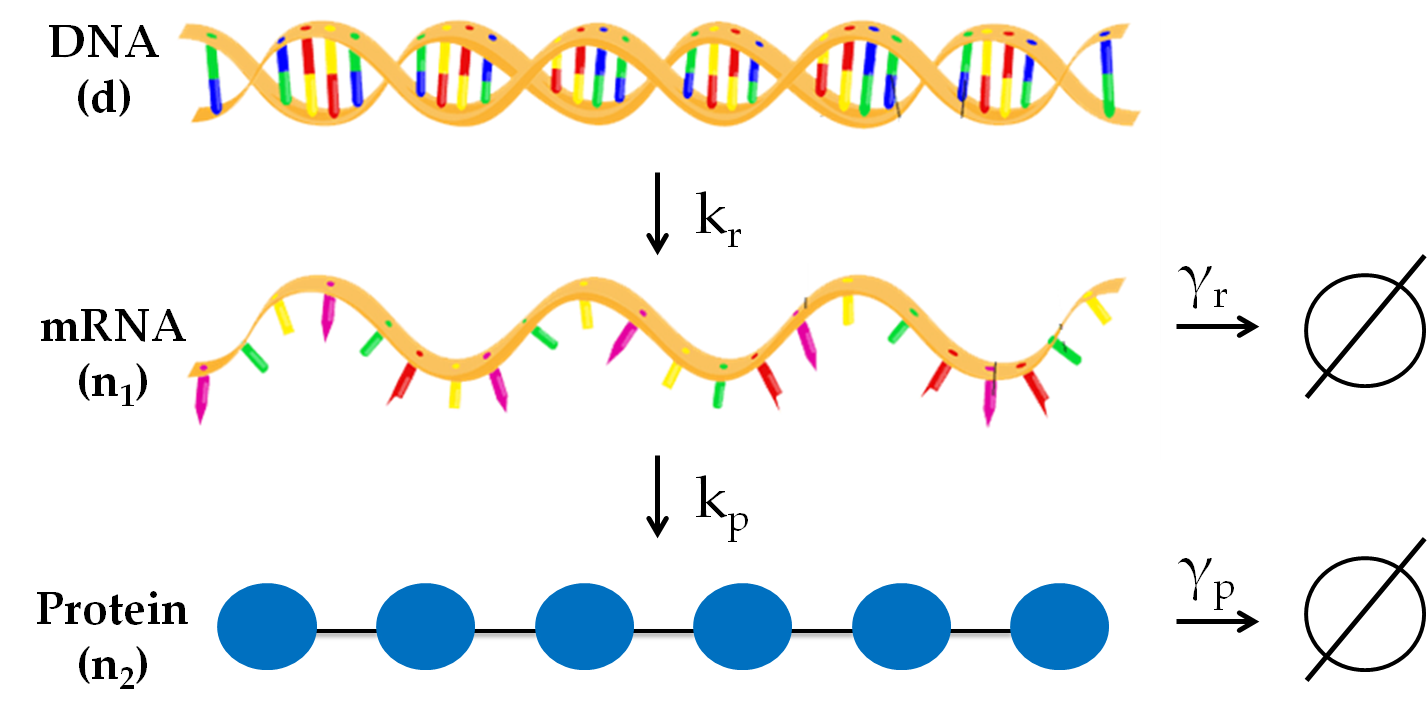
\includegraphics[width=10cm]{mas-dogma}
  \caption[Model of gene expression for a single gene]{\label{fig:mas-dogma} Steps of gene expression considered in the model.}
\end{figure}

The equations describing these processes are therefore given by

\begin{align}
  \dot{n_1}(t) &= k_rd-\gamma_rn_1(t), \label{eq:1}\\
  \dot{n_2}(t) &= k_pn_1(t)-\gamma_pn_2(t). \label{eq:2}
\end{align}

In matrix notation, they can be written as

\begin{equation}
  \label{eq:matdet}
  \mathbf{\dot{n}} = \left( \mathbf{A} - \mathbf{\Gamma} \right) \mathbf{n},
\end{equation}

where $\mathbf{n}^T=(d,n_1,n_2)$ is the vector of chemical species and the matrices $\mathbf{A}$ and $\mathbf{\Gamma}$ are defined as

\begin{eqnarray}
  \mathbf{A} &=
  \begin{pmatrix}
    0 & 0 & 0 \\
    k_r & 0 & 0 \\
    0 & k_p & 0
  \end{pmatrix},\quad \quad
  \mathbf{\Gamma} &=
  \begin{pmatrix}
    0 & 0 & 0 \\
    0 & \gamma_r & 0 \\
    0 & 0 & \gamma_p
  \end{pmatrix}.
\end{eqnarray}

Hence, $\mathbf{A}$ contains the creation rates and represents how each rate depends on the different species.

From eqs. \ref{eq:1} and \ref{eq:2} can be deduced that on steady state

\begin{align}
  \langle n_1 \rangle &= \frac{k_r}{\gamma_r}, \label{eq:ssr} \\
  \langle n_2 \rangle &= \frac{k_p}{\gamma_p} \langle n_1 \rangle = \frac{k_pk_r}{\gamma_p\gamma_r} \label{eq:ssp}.
\end{align}

But these are numbers of molecules which are discrete, and on that discreteness lies part of the stochastic behaviour of those kind of systems. The molecules are created and degradated one at a time at a certain average rate but the timing between each creation or degradation should not match exactly the rates. 

To model the intrinsic noise, we will consider each value of $\mathbf{n}$ as a possible state for the system. There are transitions between the possible states which are proportional to the rates of creation and degradation as can be seen on figure \ref{fig:mas-trans_single}.

\begin{figure}[H]
  \centering
  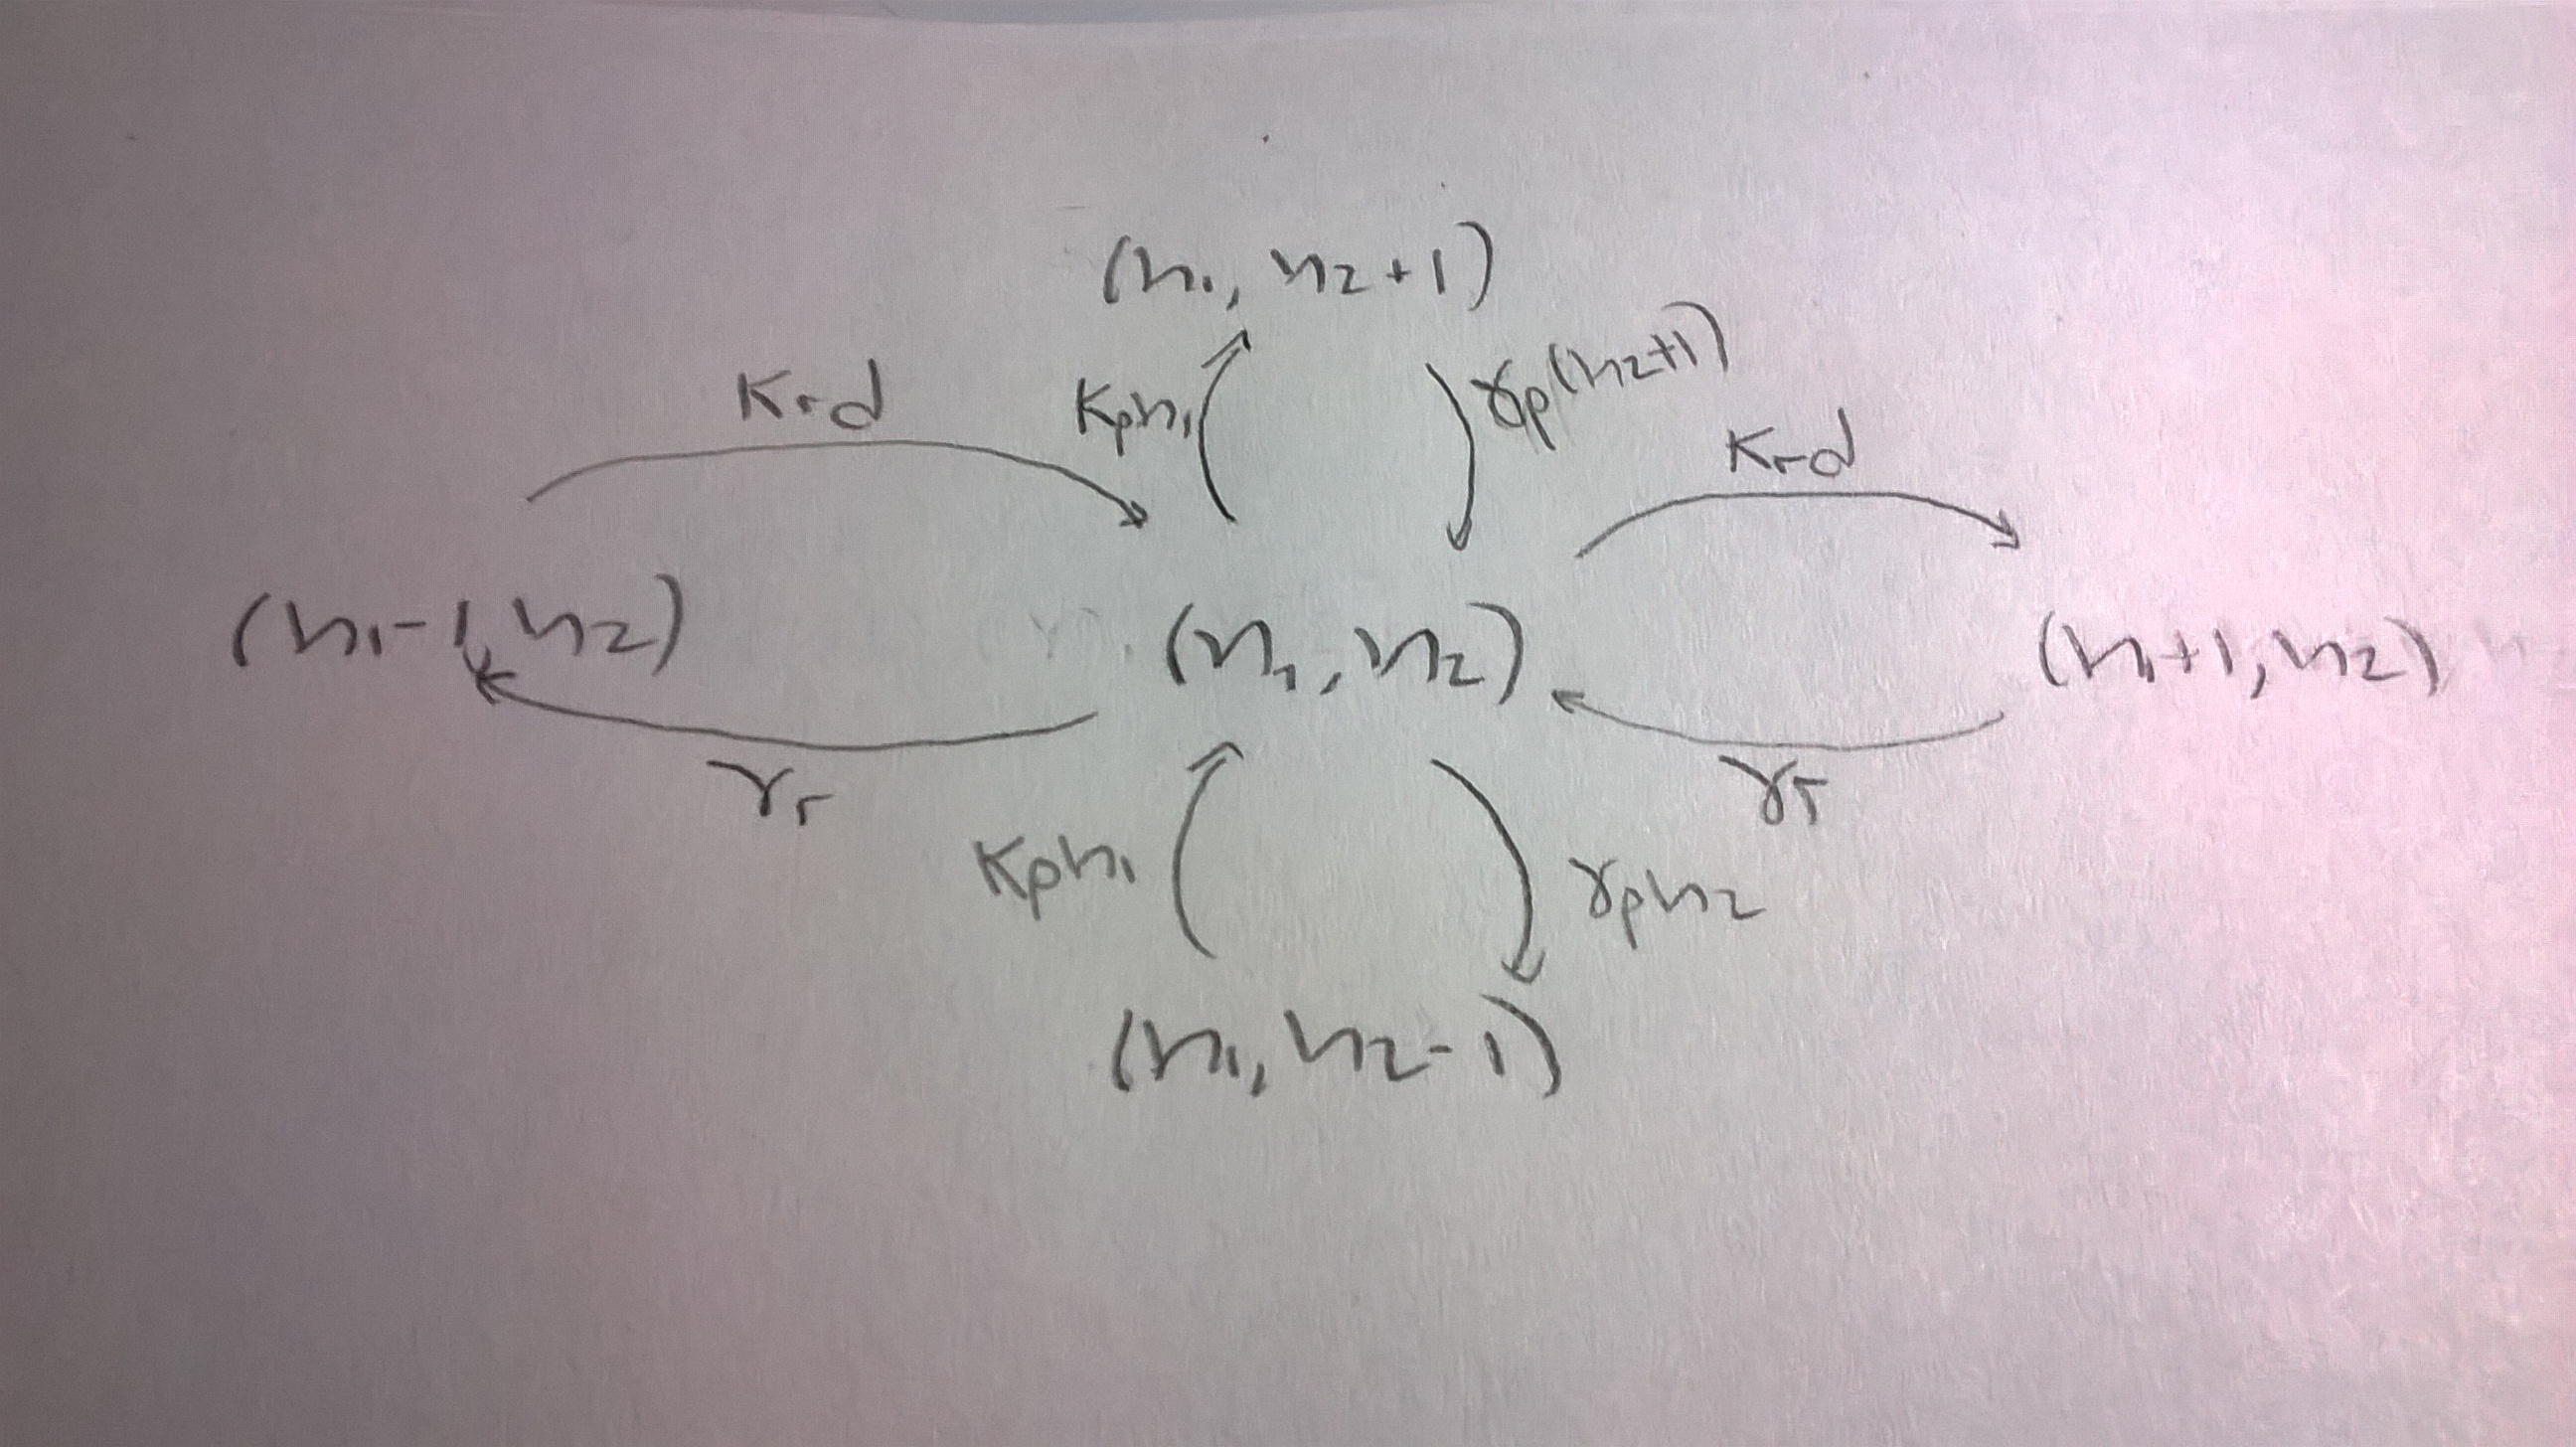
\includegraphics[width=8cm]{mas-trans_single}
  \caption[Transitions between states for a single gene]{\label{fig:mas-trans_single} Scheme of the possible transitions involving $n_1$ RNA molecules and $n_2$ protein molecules.}
\end{figure}

The transitions shown in figure \ref{fig:mas-trans_single} are the ways in which the vector $\mathbf{n}$ can change from or to $(d,n_1,n_2)$. According to this, the so called master equation can be written

\begin{equation}
  \label{eq:master}
  \begin{split}
    \frac{dp(n_1,n_2,t)}{dt} &= k_rdp(n_1-1,n_2,t) - k_rdp(n_1,n_2,t)\\
&+ k_pn_1p(n_1,n_2-1,t) - k_pn_1p(n_1,n_2,t)\\
&+ \gamma_r(n_1+1)p(n_1+1,n_2,t) - \gamma_rn_1p(n_1,n_2,t)\\
&+ \gamma_p(n_2+1)p(n_1,n_2+1,t) - \gamma_pn_2p(n_1,n_2+1,t)
  \end{split}
\end{equation}

Notice that the first term refers to a transition from state $(n_1-1,n_2,t)$ to $(n_1,n_2,t)$ via a creation of a RNA molecule, whereas the second term involves a transition $(n_1,n_2,t) \rightarrow (n_1+1,n_2,t)$ also by a creation of RNA. The third and fourth terms have a similar meaning but related to protein creation. The other terms refer to transitions due to degradation.

Multiplying by $z_1^{n_1}z_2^{n_2}$ and summing over $n_1$ and $n_2$, both from $0$ to $\infty$ we obtain, recalling the definition of the moment generating function (the time dependence and the upper limit of the sum are not shown for simplicity).

\begin{equation*}
\sum_{\mathclap{n_1=0,n_2=0}} z_1^{n_1}z_2^{n_2}f(n_1-1,n_2) = \sum_{\mathclap{n_1=-1,n_2=0}}z_1^{n_1+1}z_2^{n_2}f(n_1,n_2)
\end{equation*}

But since $n_1$ represents number of molecules, it must be a positive quantity. Hence $f(-1,n_2)=0$ and the last sum can be taken from $n_1=0$ getting

\begin{equation}
\label{eq:mom1}
z_1 \sum_{\mathclap{n_1=0,n_2=0}}z_1^{n_1}z_2^{n_2}f(n_1,n_2) = z_1F(z_1,z_2).
\end{equation}

For the second term of eq. \ref{eq:master} the result is trivial, for the third term we get

\begin{equation*}
\sum_{\mathclap{n_1=0,n_2=0}}n_1f(n_1,n_2-1) = \sum_{\mathclap{n_1=0,n_2=-1}}n_1z_1^{n_1}z_2^{n_2+1}f(n_1,n_2).
\end{equation*}

Using the same argument as above, $f(n_1,-1) = 0$. Rearranging we get

\begin{equation}
z_1 z_2 \sum_{\mathclap{n_1=0,n_2=0}} z_1^{n_1-1}z_2^{n_2}f(n_1,n_2) = z_1 z_2 \frac{\partial F(z_1,z_2)}{\partial z_1}.
\end{equation}

For the fifth term

\begin{equation}
\label{eq:mom4}
\begin{split}
\sum_{\mathclap{n_1=0,n_2=0}}(n_1+1)z_1^{n_1}z_2^{n_2}f(n_1+1,n_2) &= \sum_{\mathclap{n_1=1,n_2=0}}n_1z_1^{n_1-1}z_2^{n_2}f(n_1,n_2)\\ 
&= z_1 \sum_{\mathclap{n_1=0,n_2=0}}n_1z_1^{n_1-1}z_2^{n_2}f(n_1,n_2) = \frac{\partial F(z_1,z_2)}{\partial z_1}.
\end{split}
\end{equation}

The other terms are treated in a similar fashion. Putting all of this together in we obtain the equation for the moment generating function $F$

\begin{equation}
\label{eq:masterF}
\begin{split}
\dot{F}(z_1,z_2,t) &= k_rd(z_1-1)F(z_1,z_2,t) + k_pz_1(z_2-1)\frac{\partial F(z_1,z_2,t)}{\partial z_1} \\
&+ \gamma_r(1-z_1)\frac{\partial F(z_1,z_2,t)}{\partial z_1} + \gamma_p(1-z_2)\frac{\partial F(z_1,z_2,t)}{\partial z_2}.
\end{split}
\end{equation}

Taking the derivative with respect to $z_1$ we obtain

\begin{equation}
\label{eq:dz1}
\begin{split}
\frac{\partial \dot{F}}{\partial z_1} &= k_rd\left( F+(z-1)\frac{\partial F}{\partial z_1} \right) + k_p(z_2-1) \left( \frac{\partial F}{\partial z_1} + z_1 \frac{\partial^2 F}{\partial z_1^2} \right)\\
&+\gamma_r\left(-\frac{\partial F}{\partial z_1}+(1-z_1)\frac{\partial^2 F}{\partial z_1^2}\right)+\gamma_p(1-z_2)\frac{\partial^2 F}{\partial z_1 \partial z_2},
\end{split}
\end{equation}

and taking the derivative of eq. \ref{eq:masterF} with respect to $z_2$

\begin{equation}
\label{eq:dz2}
\begin{split}
\frac{\partial \dot{F}}{\partial z_2}&=k_rd(z_1-1)\frac{\partial F}{\partial z_2} + k_pz_1\left(\frac{\partial F}{\partial z_1} + (z_2-1)\frac{\partial^2 F}{\partial z_1 \partial z_2} \right)\\
&+ \gamma_r(1-z_1)\frac{\partial^2 F}{\partial z_1 \partial z_2} + \gamma_p\left(-\frac{\partial F}{\partial z_2}+(1-z_2)\frac{\partial^2 F}{\partial z_2^2}\right).
\end{split}
\end{equation}

Evaluating eqs. \ref{eq:dz1} and \ref{eq:dz2} at $z_1 = z_2 = 1$ and using properties (FILL) we obtain the deterministic equations

\begin{align*}
\dot{\langle n_1 \rangle}&= k_rd - \gamma_r \langle n_1 \rangle,\\
\dot{\langle n_2 \rangle}&= k_p\langle n_1 \rangle - \gamma_p \langle n_2 \rangle.
\end{align*}

Therefore, the averages follow the deterministic behavior given by eqs. \ref{eq:1} and \ref{eq:2}, as expected. The steady state values are given by eqs. \ref{eq:ssr} and \ref{eq:ssp}.

Differentiating eq. \ref{eq:dz1} with respect to $z_2$, eq. \ref{eq:dz1} with respect to $z_1$ and eq. \ref{eq:dz2} with respect to $z_2$ and evaluating at $z_1 = z_2 = 1$ we obtain, respectively

\begin{align}
\dot{\langle n_1n_2\rangle} &= k_rd\langle n_2 \rangle + k_p\left(\langle n_1\rangle + \langle n_1(n_1-1) \rangle \right) - \left( \gamma_r + \gamma_p \right)\langle n_1n_2 \rangle,\label{eq:dz1z2}\\
\dot{\langle n_1(n_1-1)\rangle} &= 2k_r\langle n_1\rangle-2\gamma_r\langle n_1(n_1-1) \rangle, \label{eq:dz1z1}\\
\dot{\langle n_2(n_2-1)\rangle} &= 2k_p\langle n_1n_2 \rangle - 2\gamma_p\langle n_2(n_2-1)\rangle. \label{eq:dz2z2}
\end{align}

We will treat the previous equations in steady state, that is, with their time derivatives equal to zero. From  eq. \ref{eq:dz1z1}, we get

\begin{equation}
\label{eq:pren1}
0 = k_rd \langle n_1 \rangle_s -\gamma_r \left(\langle n_1^2 \rangle_s - \langle n_1 \rangle_s \right) \Rightarrow \langle n_1^2 \rangle_s = \frac{k_rd}{\gamma_r}\langle n_1 \rangle_s + \langle n_1 \rangle_s = \langle n_1 \rangle_s^2 + \langle n_1 \rangle_s.
\end{equation}

Therefore, in steady state $\sigma_1^2 = \langle n_1 \rangle$ and the Fano factor and the coefficient of variation are given by (FILL)

\begin{equation}
\label{noise1}
\boxed{\nu_1 = 1}, \quad\quad \boxed{\eta_1^2 = \frac{1}{\langle n_1 \rangle}}.
\end{equation}

Which is characteristic of a Poisson process, as expected because ... (TODO).

From eq. \ref{eq:dz1z2} we have

\begin{equation*}
0 = k_rd \langle n_2 \rangle_s + k_p \langle n_1^2 \rangle_s - (\gamma_p + \gamma_r) \langle n_1n_2 \rangle_s \Rightarrow \langle n_1n_2 \rangle_s  = \frac{k_rd\langle n_2\rangle_s+k_p\langle n_1^2\rangle_s}{\gamma_r+\gamma_p}.
\end{equation*}

But from eq. \ref{eq:pren1} and \ref{eq:ssp},
\begin{equation}
\langle n_1^2 \rangle_s = \langle n_1 \rangle_s\left( \langle n_1 \rangle_s+1\right) = \frac{\gamma_p}{k_p}\langle n_2 \rangle_s\left(\langle n_1\rangle_s + 1\right),
\end{equation}

thus, the covariance is given by

\begin{align*}
\langle n_1n_2 \rangle_s - \langle n_1 \rangle_s\langle n_2\rangle_s &= \langle n_2 \rangle_s \left(\frac{k_rd+\gamma_p\left(\langle n_1\rangle_s+1\right)}{\gamma_r+\gamma_p}-\langle n_1\rangle_s\right)\\
&=\langle n_2\rangle_s\frac{k_rd+\gamma_p-\gamma_r\langle n_1\rangle_s}{\gamma_r+\gamma_p}.
\end{align*}

From eq. \ref{eq:ssr} the first and fourth term of the denominator cancel out, therefore

\begin{equation}
\label{eq:cov12}
\boxed{\text{cov}(n_1,n_2)_s = \langle n_2 \rangle_s\frac{1}{1+\frac{\gamma_r}{\gamma_p}}}.
\end{equation}

From eq. \ref{eq:dz2z2} we have in steady state

\begin{equation*}
kp\langle n_1n_2\rangle_s = \gamma_p\langle n_2^2\rangle_s-\gamma_p\langle n_2\rangle_s
\end{equation*}

Replacing eq. \ref{eq:cov12} in the previous equation we get after rearranging

\begin{align*}
\langle n_2^2\rangle_s &= \frac{k_p}{\gamma_p}\left(\langle n_1 \rangle_s\langle n_2\rangle_s + \frac{\langle n_2\rangle_s\gamma_p}{\gamma_r+\gamma_p}\right) + \langle n_2 \rangle_s\\
&=\langle n_2^2\rangle_s+\frac{k_p\langle n_2\rangle_s}{\gamma_r+\gamma_p}+\langle n_2 \rangle_s.
\end{align*}

Hence substracting $\langle n_2\rangle_s^2$ from the previous equation we obtain, in steady state,

\begin{equation}
\sigma_2^2 = \langle n_2\rangle\left(\frac{\nicefrac{k_p}{\gamma_r}}{1+\nicefrac{\gamma_p}{\gamma_r}}+1\right).
\end{equation}

Therefore, the noise in steady state is given by

\begin{equation}
\label{noise2}
\boxed{\nu_2 = \frac{\nicefrac{k_p}{\gamma_r}}{1+\nicefrac{\gamma_p}{\gamma_r}}+1}, \quad \quad \boxed{\eta_2^2 = \frac{1}{\langle n_2\rangle}\left(\frac{\nicefrac{k_p}{\gamma_r}}{1+\nicefrac{\gamma_p}{\gamma_r}}+1\right)}.
\end{equation}

As can be noticed, the noise in the proteins is bigger than Poissonian. If we define $b\coloneqq \nicefrac{k_p}{\gamma_r}$ and taking the degradation rate for a protein to be much smaller than for RNA, we have $\nicefrac{\gamma_p}{\gamma_r} \ll 1$ therefore the noise reduces to

\begin{equation}
\label{eq:noise2a}
\boxed{\nu_2 = b+1}, \quad \quad \boxed{\eta_2^2 = \frac{1}{\langle n_2\rangle}\left(b+1\right)}.
\end{equation}

\begin{figure}[H]
  \centering
  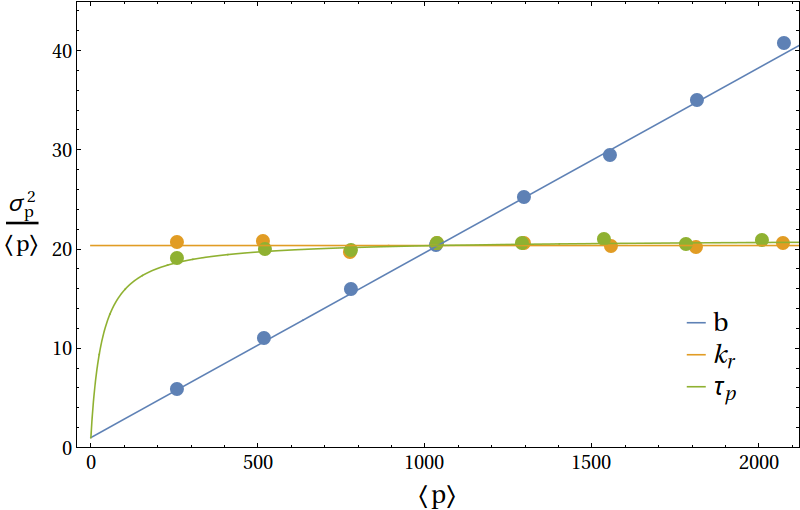
\includegraphics[width=10cm]{mas-sim_simple}
  \caption[Noise in proteins: comparing analytical results and simulations]{\label{fig:mas-sim_simple} Comparison between the results of the simulations and the analytical results given by eq. \ref{eq:noise2a}. The legend indicates which parameter is varied while the others are fixed.}
\end{figure}

CONCLUSION IMPORTANT.

\section{Several species with linear interactions}

\vspace{5cm}
Figure \ref{fig:mas-trans_single} and eq. \ref{eq:master} can be generalized according to eq. \ref{eq:matdet} to obtain \ref{fig:mas-trans_many}

\begin{figure}[H]
  \centering
  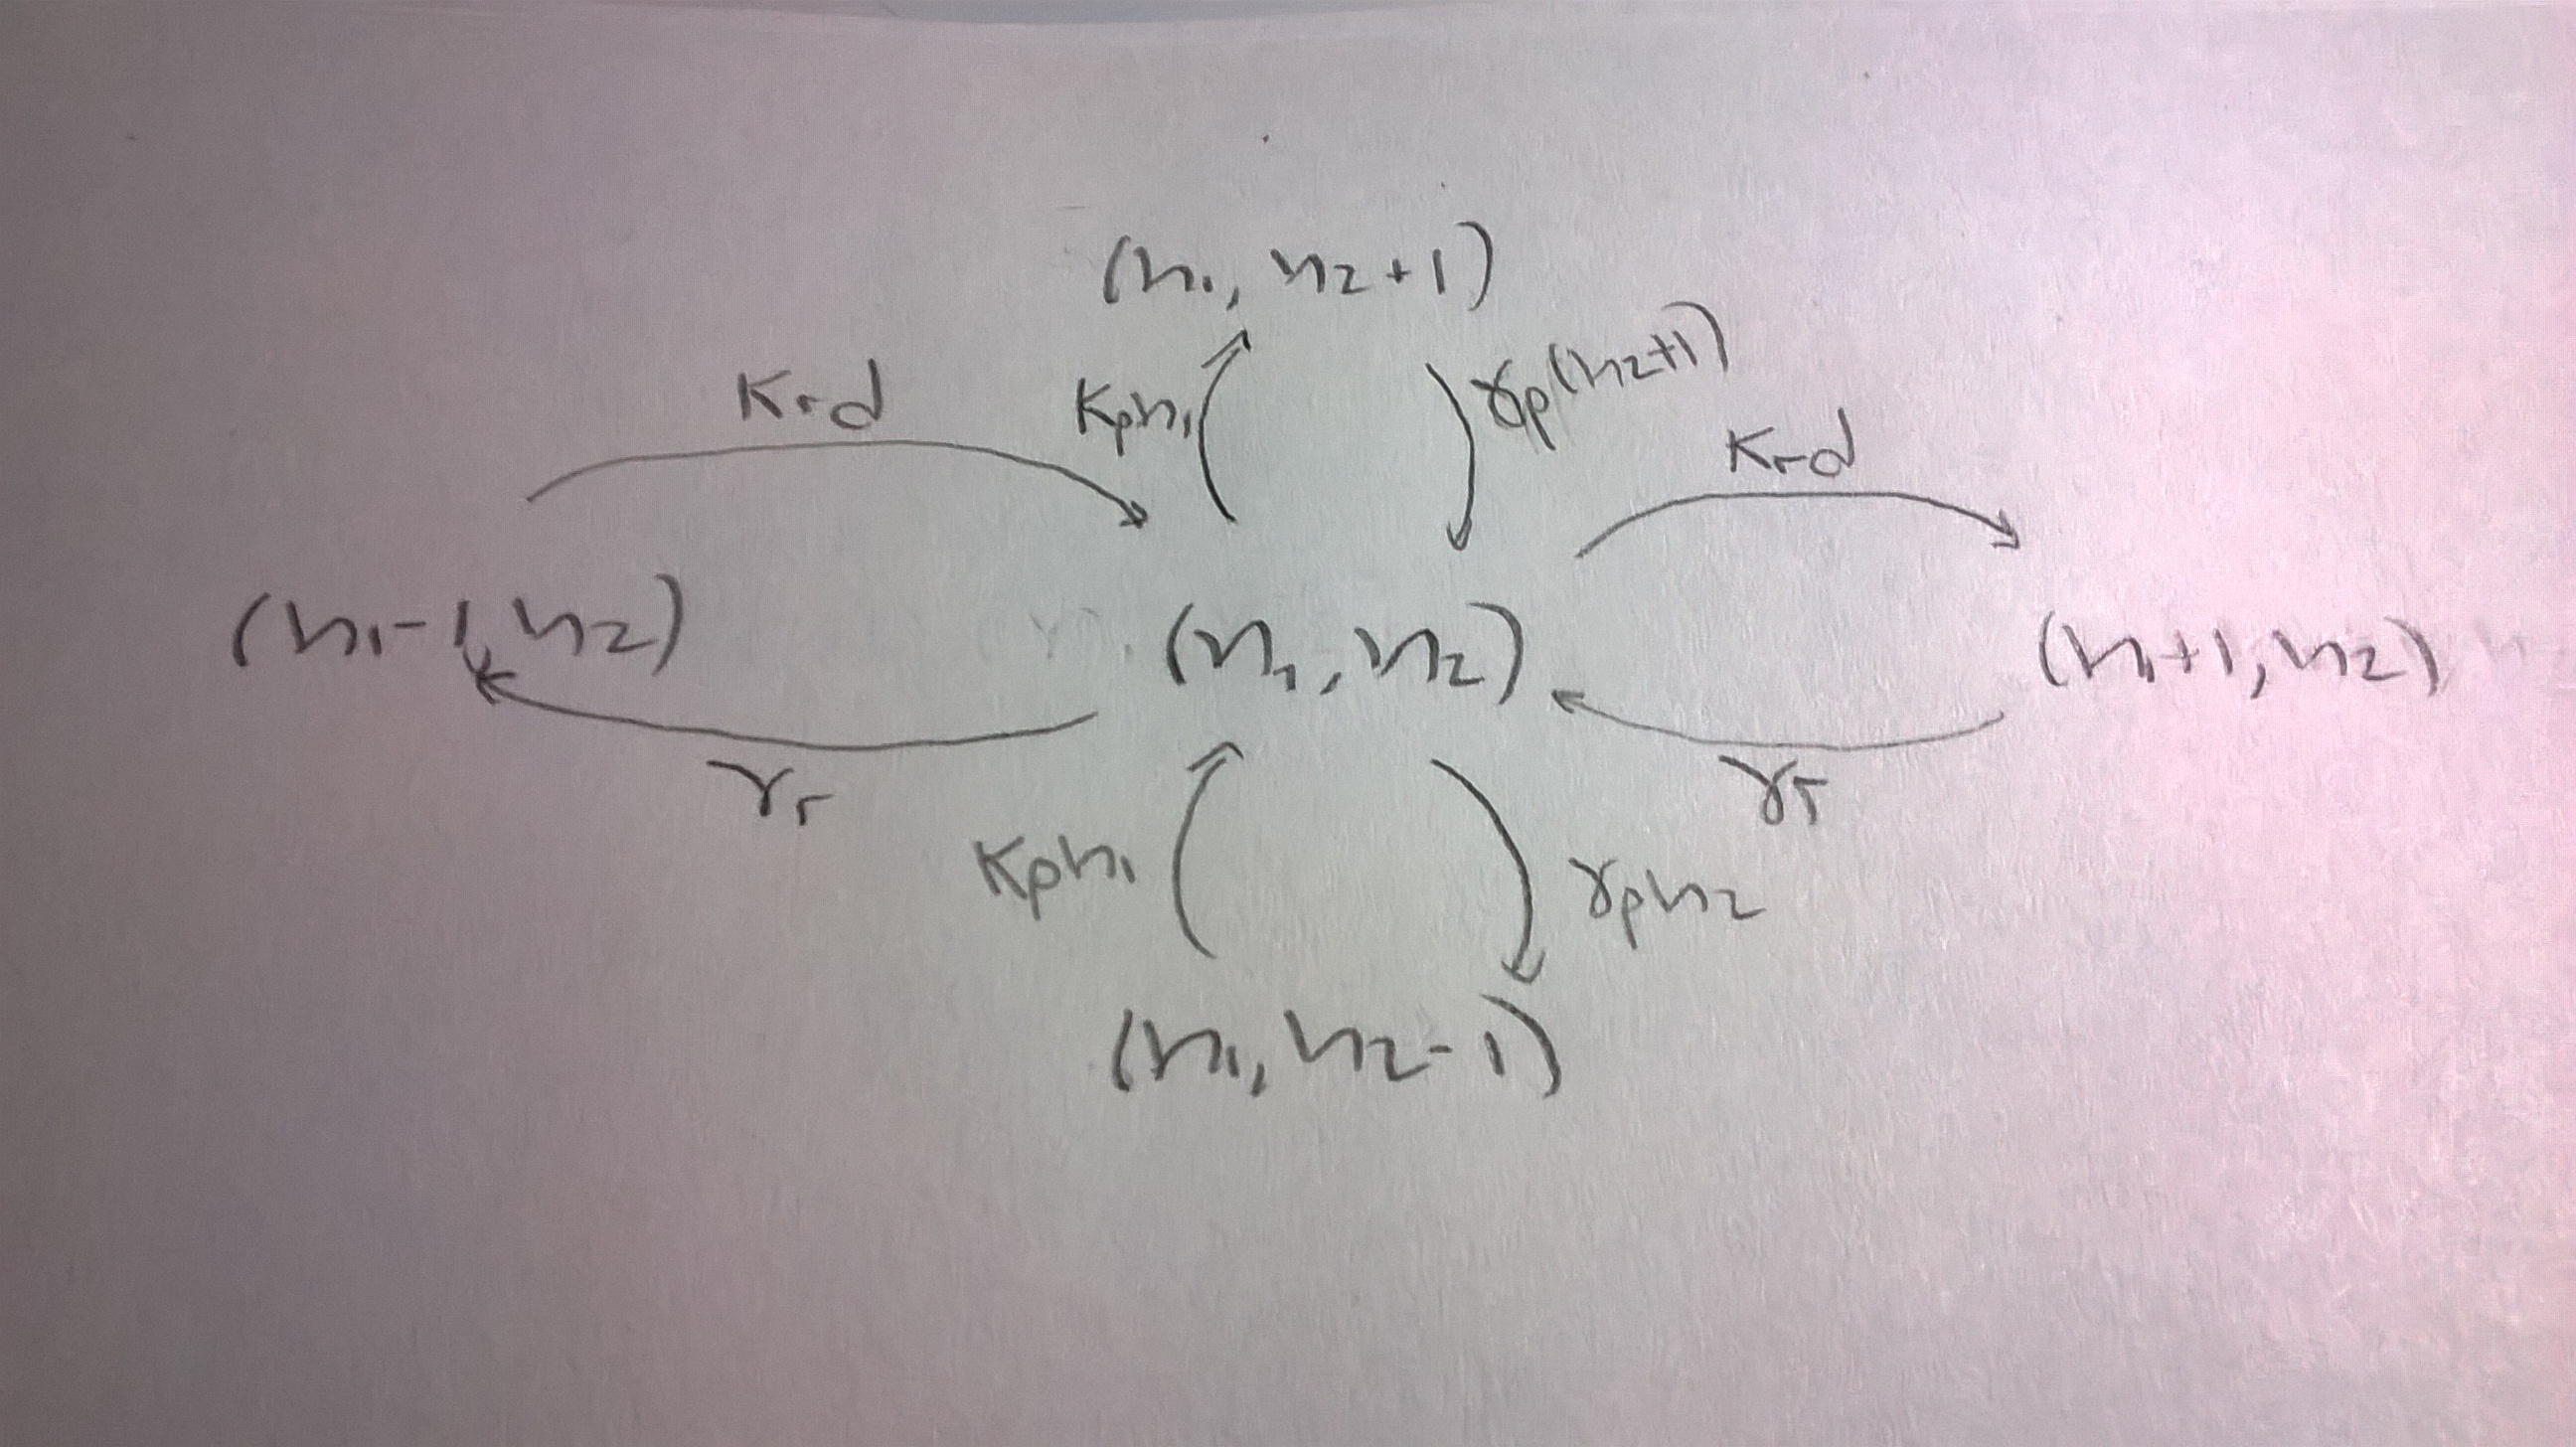
\includegraphics[width=9cm]{mas-trans_many}
  \caption[Transitions between states in general] {\label{fig:mas-trans_many} Scheme of the possible transitions in the case of three species.}
\end{figure}

The master equation can thus be written as (NOTATION, EXPLAIN THE LIMITS OF THE SUM)

\begin{equation}
\label{eq:masterg1}
\dot{f}(n_i) =  \sum_i\left(\sum_j A_{ij}n_j \left( f(n_i-1) - f(n_i) \right) + \sum_j \Gamma_{ij}((n_j+1)f(n_i+1)-n_jf(n_i))\right)
\end{equation}

Decaying is usually dependent on the quantity of the same molecule, assuming this the matrix $\Gamma$ becomes diagonal, i.e. $\Gamma_{ij}=\delta_{ij}\Gamma_j$. With this eq. \ref{eq:masterg1} becomes

\begin{equation}
\label{eq:masterg2}
\dot{f}(n_i) =  \sum_i\left(\sum_j A_{ij}n_j \left( f(n_i-1) - f(n_i) \right) + \Gamma_{i}((n_i+1)f(n_i+1)-n_if(n_i))\right).
\end{equation}

To get an equation for the moment generating functions, we multiply by $z_1^{n_1}\dotsm z_N^{n_N}$ and sum over $n_1,\dotsc n_N$, all from $0$ to $\infty$. For the first term we get an expression like the following (for a fixed $i$) (OJO ABUSE OF NOTATION, SAY LIMITS OF SUM, DEFINE EXPLICITLY ALL Zs?)

\begin{equation}
\label{eq:momg1}
\sum n_j z_1^{n_1}\dotsm z_i^{n_i}\dotsm z_j^{n_j}\dotsm z_N^{n_N} f(n_i) = z_iz_j\sum n_jz_j^{n_j-1}z_i^{n_i}f(n_i) = z_iz_j\frac{\partial F}{\partial z_j}. 
\end{equation} 

Where the same trick done previously on eqs. \ref{eq:mom1} - \ref{eq:mom4} were used. For the second term, similarly to the previous one

\begin{equation}
\label{eq:momg2}
\sum n_jz_j^{n_j}z_i^{n_i}f(n_i) = z_j\frac{\partial F}{\partial z_j}.
\end{equation}

For the third and fourth terms

\begin{equation}
\label{eq:momg3}
\sum (n_i+1)z_i^{n_i}f(n_i+1) = \sum n_i z_i^{n_i-1}f(n_i) = \frac{\partial F}{\partial z_i}.
\end{equation}

\begin{equation}
\label{eq:momg4}
\sum n_iz_i^{n_i}f(n_i) = z_i\frac{\partial F}{\partial z_i}.
\end{equation}

Replacing eqs. \ref{eq:momg1} - \ref{eq:momg4} in eq. \ref{eq:masterg2} we obtain the equation for the moment generating function

\begin{equation}
\dot{F} = \sum_i\left( z_i\sum_jA_{ij}\frac{\partial F}{\partial z_j} - \sum_jA_{ij} z_j \frac{\partial F}{\partial z_j} + \Gamma_i\frac{\partial F}{\partial z_i} - \Gamma_iz_i\frac{\partial F}{\partial z_i}\right),
\end{equation}

which after factoring becomes

\begin{equation}
\label{eq:momg}
\dot{F} = \sum_i (z_i-1)\left(\sum_jA_{ij} z_j \frac{\partial F}{\partial z_j} - \Gamma_i\frac{\partial F}{\partial z_i}\right).
\end{equation}

We have to differentiate it and use the properties (REF) to obtain equations for the moments, differentiating with respect to $z_l$

\begin{equation}
\begin{split}
\frac{\partial \dot{F}}{\partial z_l} &= \sum_i\left[(z_i-1)\left[\sum_jA_{ij}\left(\delta_{jl}\frac{\partial F}{\partial z_j}+z_j\frac{\partial^2 F}{\partial z_j\partial z_l}\right)-\Gamma_i\frac{\partial^2 F}{\partial z_i\partial z_l}\right]\right.\\
&+\left.\delta_{il}\left(\sum_jA_{ij}z_j\frac{\partial F}{\partial z_j}-\Gamma_i\frac{\partial F}{\partial z_i}\right)\right].
\end{split}
\end{equation}

\begin{equation}
\begin{split}
\frac{\partial \dot{F}}{\partial z_l} &= \sum_i(z_i-1)\left[A_{il}\frac{\partial F}{\partial z_l}+\sum_jA_{ij}z_j\frac{\partial^2 F}{\partial z_j\partial z_l}-\Gamma_i\frac{\partial^2 F}{\partial z_i\partial z_l}\right]\\
&+\sum_jA_{lj}z_j\frac{\partial F}{\partial z_j}-\Gamma_l\frac{\partial F}{\partial z_l}.
\end{split}
\end{equation}

Evaluando en $z_i=0$ para todo $i=1,\dotsc,N$ obtenemos usando las propiedades (CITAR)

\begin{equation}
\dot{\langle n_l \rangle} = \sum_jA_{lj}\langle n_j\rangle-\Gamma_l\langle n_l\rangle.
\end{equation}

Which can be written in matrix form

\begin{equation}
\dot{\langle \mathbf{n}\rangle} = (\mathbf{A}-\mathbf{\Gamma})\langle \mathbf{n}\rangle.
\end{equation}

Which is the same as  eq. (REF), as expected. Now differentiating again with respect to $z_m$ and some algebra

\begin{equation}
\begin{split}
\frac{\partial^2 \dot{F}}{\partial z_l \partial z_m} &= \sum_i(z_i-1) \left(A_{im}\frac{\partial^2F}{\partial z_i \partial z_m} + \sum_jA_{ij}z_j\frac{\partial^3F}{\partial z_j \partial z_l \partial z_m}+A_{il}\frac{\partial^2F}{\partial z_l\partial z_m} - \Gamma_i\frac{\partial^3F}{\partial z_i \partial z_l \partial z_m}   \right)\\
&+\sum_jA_{mj}z_j\frac{\partial^2F}{\partial z_j\partial z_l}+A_{ml}\frac{\partial F}{\partial z_l} - \Gamma_m\frac{\partial^2F}{\partial z_l\partial z_m} + A_{lm}\frac{\partial F}{\partial z_m} + \sum_jA_{lj}z_j\frac{\partial^2F}{\partial z_j\partial z_m}-\Gamma_l\frac{\partial^2F}{\partial z_l\partial z_m}.
\end{split}
\end{equation}

Evaluating at $z_i=1$ for all $i$ we obtain

\begin{equation}
\frac{\partial^2\dot{F}}{\partial z_l \partial z_m} = \sum_jA_{mj}z_j\frac{\partial^2F}{\partial z_j\partial z_l}+A_{ml}\frac{\partial F}{\partial z_l} - \Gamma_m\frac{\partial^2F}{\partial z_l\partial z_m} + A_{lm}\frac{\partial F}{\partial z_m} + \sum_jA_{lj}z_j\frac{\partial^2F}{\partial z_j\partial z_m}-\Gamma_l\frac{\partial^2F}{\partial z_l\partial z_m}.
\end{equation}

Which can be rewritten as

\begin{equation}
  \begin{split}
    \frac{\partial^2\dot{F}}{\partial z_l \partial z_m} &= \sum_j\left(A_{mj}z_j-\Gamma_{mj}\right)\frac{\partial^2F}{\partial z_j\partial z_l} + \sum_jA_{mj}\delta_{jl}\frac{\partial F}{\partial z_j}\\
&+\sum_j\left(A_{lj}z_j-\Gamma_{lj}\right)\frac{\partial^2F}{\partial z_j\partial z_m} + \sum_jA_{lj}\delta_{jm}\frac{\partial F}{\partial z_j}.
  \end{split}
\end{equation}

Which is valid for all $l$ and $m$, evaluating at $z_i=1$ for all $i$ we get in matrix form

%\frac{\partial^2F}{\partial z_l \partial z_m}

\begin{equation}
  \boxed{\nabla\nabla^T\dot{F}|_1 = \left(\left(\mathbf{\Gamma} - \mathbf{A}\right)\nabla\nabla^TF|_1 - \mathbf{A}\mathbf{\Theta} F|_1\right)+\left(\left(\mathbf{\Gamma} - \mathbf{A}\right)\nabla\nabla^TF|_1 - \mathbf{A}\mathbf{\Theta} F|_1\right)^T}
\end{equation}

Where $\Theta_{ij} \coloneqq \delta_{ij}\frac{\partial}{\partial z_i}$. The set of linear equations can be solved for the moments and correlation using a computer program.

\section{Several species with non-linear interactions - Negative autorregulation}

\begin{figure}[H]
  \centering
  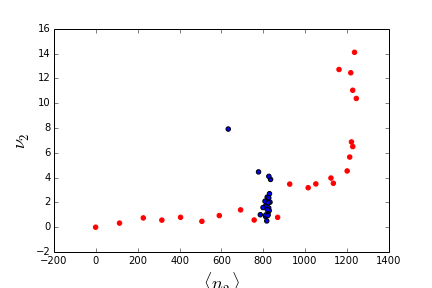
\includegraphics[width=9cm]{mas-sim_autorreg}
  \caption[Autorregulation simulation results]{\label{fig:mas-sim_autorreg} Simulation for the case of autorregulation}
\end{figure}
